\documentclass[a4paper,oneside,12pt]{book}

%----------------------------------------------------------------------------------------
%	README!
%   Welcome. It's worth having a read through this file
%   to set up the broad parameters, such as the name of
%   the degree, the school/department, the type of work
%   (dissertation/Final Year Project/report, etc. as well
%   as your details.
%----------------------------------------------------------------------------------------

%----------------------------------------------------------------------------------------
%	COVER PAGE
%   The cover page is laid out in title/title.tex. You can choose a color
%   or black and white logo
%----------------------------------------------------------------------------------------

%----------------------------------------------------------------------------------------
%	THESIS INFORMATION
%   Put title, author name, supervisor name, degree, type of work, school, department in here
%   It will be used for the title page and the embedded PDF information
%----------------------------------------------------------------------------------------

\newcommand{\thesistitle}{MERIT.jl: Julia's Version} % Your thesis title, this is used in the title and abstract
\newcommand{\degree}{MAI (Electronic and Computer Engineering)} % Replace with your degree name, this is used in the title page and abstract
\newcommand{\typeofthesis}{Final Year Project} % dissertation, Final Year Project, report, etc.
\newcommand{\authorname}{Aaron Dinesh} % Your name, this is used in the title page and PDF stuff
%% Do not put your Student ID in the document, as TCD will not publish
%% documents that contain both your name and your Student ID.
\newcommand{\supervisor}{Associate Prof. Declan O'Loughlin} % replace with the name of your supervisor
%\newcommand{\cosupervisor}{Dr. Alex Lee} % replace with the name of your co-supervisor if you have one
\newcommand{\keywords}{Microwave Imaging, Breast Imaging, Julia} % Replace with keywords for your thesis
\newcommand{\school}{\href{https://www.tcd.ie/Engineering/}{School of Engineering}} % Your school's name and URL, this is used in the title page
%Edited by HS for engineering

%% Comment out the next line if you don't want a department to appear
\newcommand{\department}{\href{https://www.tcd.ie/eleceng/}{Electronic Engineering}} % Your research group's name and URL, this is used in the title page


%% Language and font encodings
\usepackage[T1]{fontenc} 
\usepackage[utf8]{inputenc}
\usepackage[english]{babel}
\usepackage{ulem}
%% Bibliographical stuff
\usepackage[]{cite}
%% Document size
%Include showframe as an option if you want to see the boxes
\usepackage[a4paper,top=2.54cm,bottom=2.54cm,left=2.54cm,right=2.54cm,headheight=16pt]{geometry}
\setlength{\marginparwidth}{2cm}
%% Useful packages
\usepackage{amsmath}
\usepackage[autostyle=true]{csquotes} % Required to generate language-dependent quotes in the bibliography
\usepackage[pdftex]{graphicx}
\usepackage[colorinlistoftodos]{todonotes}
\usepackage[colorlinks=true, allcolors=black]{hyperref}
\usepackage{hyperxmp}
\usepackage{caption} % if no caption, no colon
\usepackage{sfmath} %use sans-serif in the maths sections too
\usepackage[parfill]{parskip}    % Begin paragraphs with an empty line rather than an indent
\usepackage{setspace} % to permit one-and-a-half or double spacing
\usepackage{enumerate} % fancy enumerations like (i) (ii) or (a) (b) and such
\usepackage{booktabs} % To thicken table lines
\usepackage{fancyhdr}
\usepackage{xcolor} % to get TCD color on headings
\usepackage{hvfloat}
\usepackage{subcaption}
\captionsetup[figure]{font={scriptsize, sf}}

\graphicspath{{./Images/}}
\numberwithin{equation}{chapter} %HS edit for (chapter.equation)
\pagestyle{plain} % Embrace simplicity!

\definecolor{tcd_blue}{RGB}{5, 105, 185}

%% For Today's Date
\renewcommand{\today}{\ifnum\number\day<10 0\fi \number\day \space%
\ifcase \month \or January\or February\or March\or April\or May%
\or June\or July\or August\or September\or October\or November\or December\fi \space%
\number \year}

%% It's personal taste but...
%% Uncomment the following block if you want your name and ID at the top of
%% (almost) every page.

%\pagestyle{fancy}
%\fancyhf{} % sets both header and footer to nothing
%\renewcommand{\headrulewidth}{0pt}
%\cfoot{\thepage}
%\ifdefined\authorid
%\chead{\it \authorname\ (\authorid)}
%\else
%\chead{\it \authorname}
%\fi
%% End of block

%% It is good practice to make your font sans-serif to improve the accessibility of your document.  Comment out the following line to disable it (but you really should not)
\renewcommand{\familydefault}{\sfdefault} %use the sans-serif font as default

%% If you insist on not using sans-serif (please don't), consider using Palatino instead of the LaTeX standard
%\usepackage{mathpazo} % Use the Palatino font by default if you prefer it to Computer Modern


%% Format Chapter headings appropriately
\usepackage{titlesec}
\titleformat{\chapter}[hang]{\normalfont\huge\bfseries\color{tcd_blue}}{\thechapter}{1cm}{}{}

\title{\thesistitle}
\author{\authorname}


\hypersetup{
   pdftitle=\thesistitle, % Set the PDF's title to your title
   pdfauthor=\authorname, % Set the PDF's author to your name
   pdfkeywords=\keywords, % Set the PDF's keywords to your keywords
   pdfsubject=\degree, % Set the PDF's keywords to your keywords
   pdfinfo={
     pdfsupervisor=\supervisor, % Set the PDF's supervisor to your supervisor
     %pdfcosupervisor=\cosupervisor, % Set the PDF's cosupervisor to your cosupervisor if using
   }
}


\frontmatter
\begin{document}

\input{ch-Title.tex}
\pagenumbering{roman}
\section*{\Huge\textcolor{tcd_blue}{Declaration}}
\vspace{1cm}
I hereby declare that this \typeofthesis\ is entirely my own work and that it has not been submitted as an exercise for
a degree at this or any other university.

\vspace{1cm}
I have read and understand the plagiarism provisions in the General Regulations of the University Calendar for the
current year, found at \url{http://www.tcd.ie/calendar}.
\vspace{1cm}

I have completed the Online Tutorial on avoiding plagiarism `Ready Steady Write', located at
\url{http://tcd-ie.libguides.com/plagiarism/ready-steady-write}.
\vspace{1cm}

I consent/do not consent to the examiner retaining a copy of the thesis beyond the examining period, should they so
wish (EU GDPR May 2018).
\vspace{1cm}

I agree that this thesis will not be publicly available, but will be available to TCD staff and students in the
University’s open access institutional repository on the Trinity domain only, subject to Irish Copyright Legislation and
Trinity College Library conditions of use and acknowledgment.  \textbf{Please consult with your supervisor on this last
item before agreeing, and delete if you do not consent}
\vspace{3cm}

Signed: \uline{\hfill Aaron Dinesh \hfill} Date: \uline{\hfill \today \hfill}

\chapter*{Abstract}
MERIT aims to provide a software framework that is robust, easy to use and performant. It implements a variety of
microwave imaging algorithms and a myriad of helper functions, all while leveraging the powerful features available in
Julia. MERIT.jl also implements a ``Scan'' abstract datatype which allows users to subtype their own specialized datatype.
Organizing the datatypes in this way means that MERIT.jl plays very well with Julia's own type hierarchy and also the
other language features that depend on this. To encourage type safety, MERIT.jl implements a lightweight Points class
which allows for efficient processing of coordinate points. In this way, collections of points won't simply be a matrix
of Floats or Ints instead, they would be a Vector of the Points type. In this way, the Julia compiler will throw an
error when Points aren't passed in the right argument, instead of providing a wrong output.      
\newpage

\section*{\Huge\textcolor{tcd_blue}{Acknowledgements}}
Thanks, Everyone!
\newpage

\listoffigures
\tableofcontents
\newpage

%%\section*{\Huge\textcolor{tcd_blue}{Nomenclature}}
%%\begin{tabular}{lp{9cm}l}
%%  A        & Area of the wing                                                               & $m^{2}$ \\
%%  B                                                                                                   \\
%%  C        & Roman letters first, with capitals\ldots                                                 \\
%%  a        & then lower case.                                                                         \\
%%  b                                                                                                   \\
%%  c                                                                                                   \\
%%  $\Gamma$ & Followed by Greek capitals\ldots                                                         \\
%%  $\alpha$ & then lowercase Greek symbols.                                                           \\
%%  $\beta$                                                                                             \\
%%  $\epsilon$                                                                                          \\
%%  TLA      & Finally, three letter acronyms and other abbreviations arranged alphabetically           \\
%%\end{tabular}
%%\vspace{2cm}
%%
%%If a parameter has a typical unit that is used throughout your report, then it should be included here on the right hand side.
%%
%%If you have a very mathematical report, then you may wish to divide the nomenclature list into functions and variables, and then sub- and super-scripts.
%%
%%If you have a large number of acronyms, check out \href{https://www.overleaf.com/learn/latex/Glossaries} to make that more robust.
%%
%%Note that Roman mathematical symbols are typically in a serif font in italics.

\mainmatter
% Maintaining separate .tex files for each chapter is good practice
\setcounter{chapter}{1}
\chapter*{Introduction}
\addcontentsline{toc}{chapter}{Introduction}
Microwave imaging has seen a rising interest in the medical field evidenced by the numerous clinical trials that are
being conducted by research groups around the world \cite{preeceMARIAM4Clinical2016, moloneyWaveliaMicrowaveBreast2021,
e.c.fearMicrowaveBreastImaging2013}. A cursory search on GitHub for software around microwave imaging yielded few useful
results, with many being specialized repositories for a particular task or performing some machine learning analysis on
microwave data. Only one repository stood out as a generalized library that provides researchers with all the tools
needed to easily test different algorithms; the MERIT toolbox developed by Dr. O'Loughlin, M. A. Elahi, E. Porter,
\textit{et al.} \cite{d.oloughlinOpensourceSoftwareMicrowave2018}. Other fields of research have seen numerous benefits
from the introduction of comprehensive open-source libraries. For example, libraries such as PsychoPy and PsyToolkit
have allowed psychology researchers to design and conduct experiments in a matter of hours by packaging common functions
in an easy-to-use library \cite{stoetPsyToolkitTestimonials}. With a rise in the number of systems that can perform
microwave imaging and the vast amounts of data being generated from these systems, it is imperative that there are a
variety of toolkits available to not only analyze data from these current systems but also from future systems. This
thesis aims to consider the following questions:
\begin{itemize}
    \item Improving the reliability of Microwave Imaging software
    \item Increasing the compatibility between systems, the data these systems generate and the software used to analyze
    this data
    \item Creating an intuitive, easily extensible and customizable library
    \item Leveraging the features of a coding language to create a performant library   
\end{itemize}
\vspace{1cm}
The rest of the report will be divided up as follows:
\begin{itemize}
    \item A review of existing microwave imaging systems
    \item A look into existing reconstruction algorithms 
    \item A discussion about the programming paradigms in Julia and their benefits for MERIT.jl and scientific computing
    in general
    \item An examination of the results and possible future work
\end{itemize}

MERIT.jl being an open-source library has all its code available on GitHub for anyone to view and amend. It can be
viewed at the following URL: \url{https://github.com/AaronDinesh/MERIT.jl}

Any files referenced in this thesis can be found in the GitHub repository.

\chapter*{Background}
\addcontentsline{toc}{chapter}{Background}
\section{Literature Review}
In order to understand the design requirements of the library, a literature review needed to be performed. The scope was
narrowed down to 3 systems that showed promise and were broadly representative of the antenna configuration that future
systems would adopt. Most systems will adopt one of the following setups
\begin{enumerate}
    \item Monostatic
    \item Leveled Multistatic
    \item Fully Multistatic
\end{enumerate}
\noindent These terms relate to the position of antennas around the breast tissue and how the resulting scan data would
be structured. \hfill \break

\subsection{MARIA M4}
The first system we will look at is the MARIA M4 system developed by Preece et al within the Electrical and Engineering
Department of the University of Bristol \cite{preeceMARIAM4Clinical2016}. This is the 4th iteration in a series of MARIA systems that evolved from a
system of 16 UWB antennas to 60 antennas in the current system. These all operate in a multistatic configuration,
meaning that any antenna in the array can listen to any other antenna in the array, an example of which can be seen in
Figure \ref{fig:MultistaticExample}. This figure shows a top-down view, however, one can imagine this being generalized
to a hemisphere of antennas around the breast. \hfill

\begin{figure}
    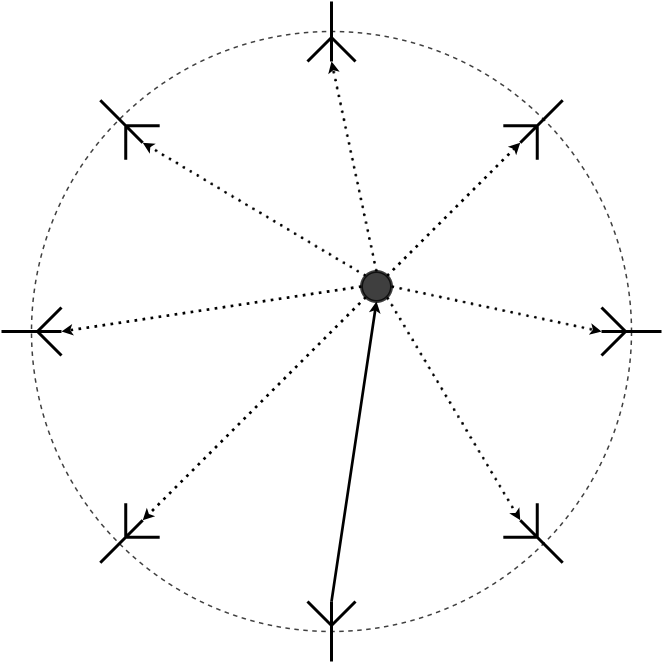
\includegraphics[width=0.3\textwidth]{multistaic.png}
    \centering
    \caption{Example of a Fully Multistatic Configuration (Top-Down)}
    \label{fig:MultistaticExample}
\end{figure}

\noindent As stated before, the MARIA M4 systems makes use of the UWB spectrum over a frequency range of 3.0 to 8.0 GHz. A
VNA was used to step through the frequencies and collect the scans from the antenna. The system exploits the inherent
symmetry in the antenna reciprocity to halve the number of channels (made of a transmitting and receiving antenna)
collected, thereby speeding up the scan time. For the MARIA M4 system, this equates to a 1770 reduction in the number of
channels collected. Figure \ref{fig:MARIAM4}, shows the antenna array used in the M4 system (a), as well as the M5
system (c) which is an integrated package.


\begin{figure}
    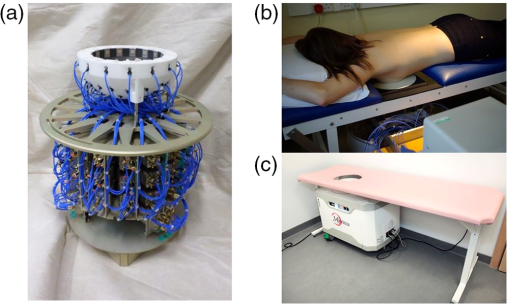
\includegraphics[width=0.5\textwidth]{MARIA_M4.png}
    \centering
    \caption{The MARIA M4 and M5 system. (a) The MARIA M4 antenna array. (b) The M4 in a clinical setting. (c) The integrated M5 package \cite{preeceMARIAM4Clinical2016}}
    \label{fig:MARIAM4}
\end{figure}

\noindent The team scanned 86 participants, with a mean age of 51.4 and a range of 24 - 78 years old. The M4 system showed a sensitivity of
74\% (64/86) when compared with the "gold-standard' of an ultrasound. The "sensitivity" was determined based on the
ability of the M4 system to localize a lesion as it correlated with the location in the ultrasound image. The research
team also divided the group into pre-/peri- and post- menopausal women and found that the sensitivity was 75\% and 73\%
respectively. However, the reliability of these results are called into question when considering the sample size of the
study. Given a sample size of 86, and assuming a normal distribution and that the results are statistically significant
($p < 0.05$, Z = 1.96), a 10.58\% margin of error was calculated. While this may not be enough to conclusively prove
that the M4 system is a viable alternative to Mammograms, it is enough to show promise. With a larger sample size, this
margin of error could be narrowed further.

\subsection{Wavelia}
The second system that was considered was the Wavelia Microwave Breast Imaging System developed by MVG Industries
\cite{moloneyWaveliaMicrowaveBreast2021}. The Wavelia system integrates the imaging system as well as the examination
bed into one complete package (Figure \ref{fig:WaveliaSystem}). The integrated package makes the Wavelia system an
appealing choice for some hospitals, however, its large size may be a barrier to adoption in some facilities where space
is a premium. \hfill \break

\begin{figure}
    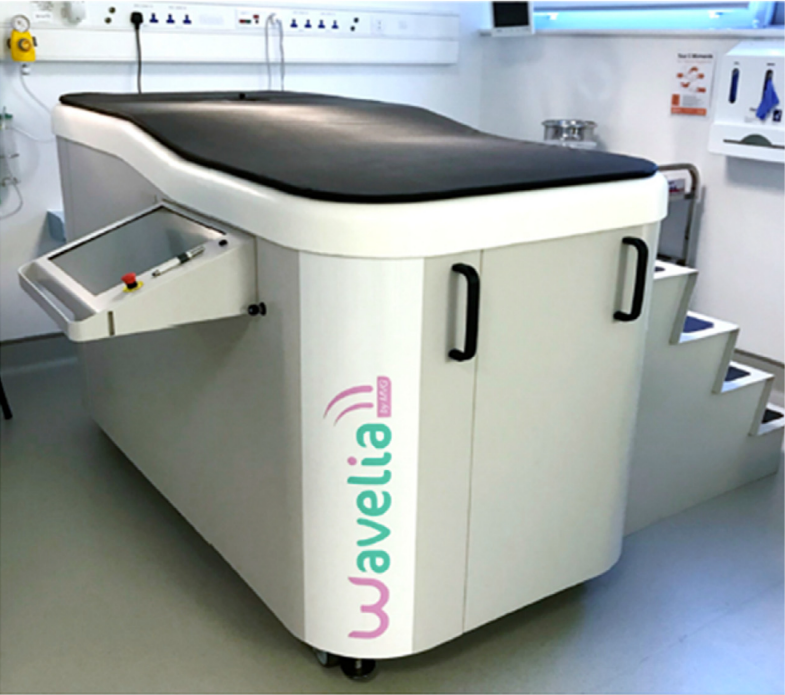
\includegraphics[width=0.5\textwidth]{Wavelia.png}
    \centering
    \caption{The Wavelia System \cite{moloneyWaveliaMicrowaveBreast2021}}
    \label{fig:WaveliaSystem}
\end{figure}

Like in the MARIA M4 system, patients lie in a prone position and place their breasts in the circular cutouts on the
bed. The system then begins to create a 3D reconstruction of the exterior of the breast using a stereoscopic camera.
This also allows for the breast volume to be explicitly calculated rather than being inferred like in the MARIA system.
The Wavelia makes use of the UWB spectrum when imaging the breast, although they opt for a narrower frequency range of
0.5 - 4.0 GHz compared to the 3.0 - 8.0 GHz range of the MARIA system. The antenna configuration, unlike the MARIA system, is an array of 18 Vivaldi-type probes arranged in a concyclic manner
on a horizontal plane. These antennas operate in a Multistatic manner and image the breast in sections parallel to the
coronal plane. The entire antenna assembly moves downwards in 5mm intervals to image the entire breast (Figure \ref{fig:LeveledMultistaticExample}). This is a
leveled multistatic system as opposed to the fully multistatic system in the MARIA M4. This leveled multistatic approach
has the benefit of a theoretically infinite vertical resolution. If the radiologist wanted a finer resolution along the
coronal plane, they would just have to tweak the array vertical step size, rather than having to manufacture an entirely
new antenna array, like in the MERIT system. This leveled approach also allows the parameters of the reconstruction
algorithm to be easily changed based on the particular section of the breast that we are imaging. The fully multistatic
approach, however, would need significant additional logic in the post-processing steps to determine which channels are
coplanar with a particular section. \hfill \break

\begin{figure}
    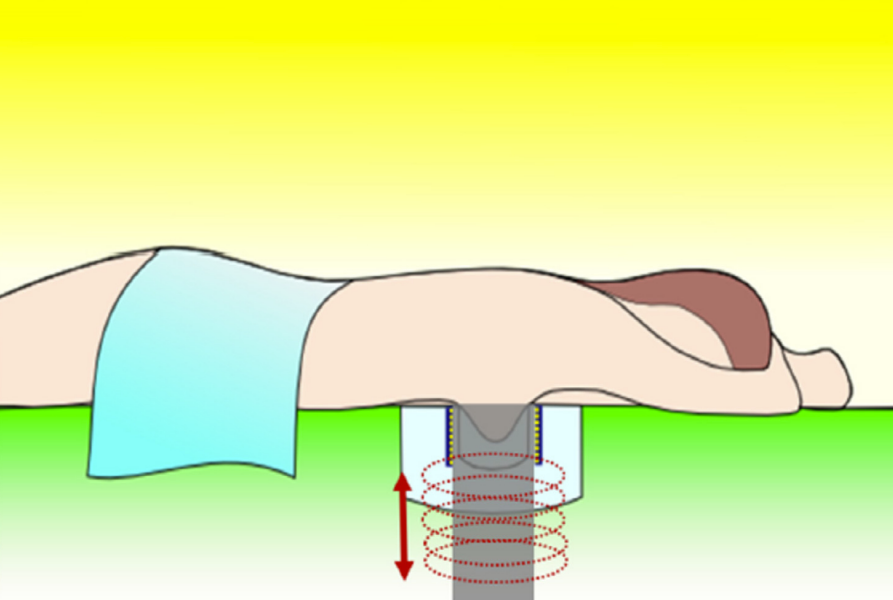
\includegraphics[width=0.5\textwidth]{LeveledMultistatic.png}
    \centering
    \caption{The Leveled Multistatic Approach of Wavelia \cite{moloneyWaveliaMicrowaveBreast2021}}
    \label{fig:LeveledMultistaticExample}
\end{figure}

\noindent The Wavelia paper \cite{moloneyWaveliaMicrowaveBreast2021} conducted a feasibility study on 25 female
participants. While the results aren't statistically significant, they do demonstrate the strengths of the Wavelia
system. 11 of the participants had a biopsy confirmed carcinoma and out of these, the Walia system detected 9 lesions,
with 7 being located to the appropriate region. Overall the system detected an abnormality in 21 of the 24 participants,
leading to a sensitivity of 87.5\%. The researchers do note some limitations of the Walia system, namely it can't detect
any lesions smaller than 10mm. This is significant since the size of the detected lesion plays a big factor when
deciding whether a lesion is cancerous or not. Another limitation of the system is that breast sizes that are too small
cannot be scanned in any great detail by the Wavelia system. Due to the patients being in the prone position, their
breast tissue needs to hang down far enough to have multiple sections of their breast be imaged by the antenna array.
The researchers are working on a subsequent system that should address all the aforementioned limitations. Overall the
participants had a positive outlook on the system. 23 out of the 25 women said that they would recommend the procedure
to other women and all of the women agreed that the information provided was clear and well understood.

\subsection{TSAR}

% note that your supervisor may have a strong opinion on the style of referencing you use. Some background is available at https://www.overleaf.com/learn/latex/Bibtex_bibliography_styles
\bibliographystyle{IEEEtran} %Changed to IEEETran by HS
%\bibliographystyle{unsrt}

\bibliography{citations.bib}
\appendix
\renewcommand{\thechapter}{A\arabic{chapter}}
\end{document}